% Author: Till Tantau
% Source: The PGF/TikZ manual
\documentclass[a4paper,11pt]{article}
\usepackage[utf8]{inputenc}
\usepackage{listings}
\usepackage{amsmath}    % need for subequations
\usepackage{graphicx}   % need for figures
\usepackage{verbatim}   % useful for program listings
\usepackage{color}      % use if color is used in text
%\usepackage{subfigure}  % use for side-by-side figures
\usepackage{hyperref}   % use for hypertext links, including those to external documents and URLs
\usepackage{url}
\usepackage{float}
\usepackage{todonotes}
\usepackage{tikz}
\usepackage{enumitem}
\usepackage{hyperref}
\usepackage{pdfpages}
\usepackage{caption}
\usepackage{subcaption}
\usepackage{listings}
\usepackage{color}
\usepackage{amsfonts}
\usepackage{latexsym}
\usepackage[T1]{fontenc} % use for allowing < and > in cleartext
\usepackage{fixltx2e}    % use for textsubscript
\usepackage[linesnumbered,boxed,ruled]{algorithm2e}
% \newcommand{\BigO}[1]{\ensuremath{\operatorname{O}\left(#1\right)}}
\newcommand{\BigO}[1]{\ensuremath{\mathop{}\mathopen{}\mathcal{O}\mathopen{}\left(#1\right)}}
\graphicspath{ {./images/} }
\definecolor{mygreen}{rgb}{0,0.6,0}
\definecolor{mygray}{rgb}{0.5,0.5,0.5}
\definecolor{mymauve}{rgb}{0.58,0,0.82}
\lstset{ %
  backgroundcolor=\color{white},   % choose the background color; you must add \usepackage{color} or \usepackage{xcolor}
  basicstyle=\footnotesize,        % the size of the fonts that are used for the code
  breakatwhitespace=false,         % sets if automatic breaks should only happen at whitespace
  breaklines=true,                 % sets automatic line breaking
  captionpos=b,                    % sets the caption-position to bottom
  commentstyle=\color{mygreen},    % comment style
  deletekeywords={...},            % if you want to delete keywords from the given language
  escapeinside={\%*}{*)},          % if you want to add LaTeX within your code
  extendedchars=true,              % lets you use non-ASCII characters; for 8-bits encodings only, does not work with UTF-8
  %frame=single,                    % adds a frame around the code
  keepspaces=true,                 % keeps spaces in text, useful for keeping indentation of code (possibly needs columns=flexible)
  keywordstyle=\color{blue},       % keyword style
  language=Octave,                 % the language of the code
  morekeywords={*,...},            % if you want to add more keywords to the set
  numbers=left,                    % where to put the line-numbers; possible values are (none, left, right)
  numbersep=5pt,                   % how far the line-numbers are from the code
  numberstyle=\tiny\color{mygray}, % the style that is used for the line-numbers
  rulecolor=\color{black},         % if not set, the frame-color may be changed on line-breaks within not-black text (e.g. comments (green here))
  showspaces=false,                % show spaces everywhere adding particular underscores; it overrides 'showstringspaces'
  showstringspaces=false,          % underline spaces within strings only
  showtabs=false,                  % show tabs within strings adding particular underscores
  stepnumber=2,                    % the step between two line-numbers. If it's 1, each line will be numbered
  stringstyle=\color{mymauve},     % string literal style
  tabsize=2,                       % sets default tabsize to 2 spaces
  %title=\lstname                   % show the filename of files included with \lstinputlisting; also try caption instead of title
}

\bibliographystyle{plain}
\begin{document}

\date{May 18th 2014\\ IT University of Copenhagen}
\title{Assignment 3 - Shading\\SIGB Spring 2014}

\author{Marcus Gregersen\\
\texttt{mabg@itu.dk}
\and Martin Faartoft\\
\texttt{mlfa@itu.dk}
\and Mads Westi\\
\texttt{mwek@itu.dk}}
\clearpage\maketitle
\thispagestyle{empty}
\setcounter{page}{1}
\newpage

% \begin{figure}[H]
% \centering
% \begin{subfigure}{.4\textwidth}
%   \centering
%   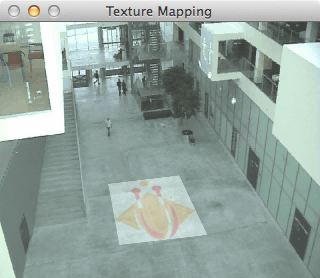
\includegraphics[width=0.8\linewidth]{groundfloor1}
%   \label{fig:floor1}
% \end{subfigure}
% \begin{subfigure}{.4\textwidth}
%   \centering
%   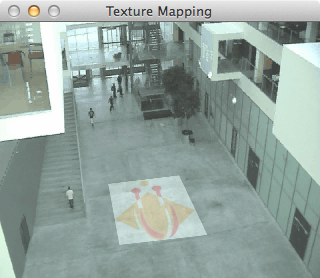
\includegraphics[width=0.8\linewidth]{groundfloor2}
%   \label{fig:floor2}
% \end{subfigure}
% \caption{Linear texture mapping to sequence}
% \label{fig:floor}
% \end{figure}

\section{Introduction}
In this report, we will implement and document a simple shader, able to render a textured cube, and shade it realistically.

\section{Back-Face Culling}
When we render the cube, at most 3 of the faces will be visible to camera, regardless of the positions of cube and camera. Attempting to render all 6 will waste a lot of performance, and furthermore require us to render the faces in the correct order, to get the correct perspective.\todo{eksempelbillede uden culling}

The idea behind back-face culling, is to calculate the dot-product between the camera view vector, and each of the face normals. If the result is negative, the face should be drawn - otherwise it faces away from the camera, and should be discarded.
\[cos(\theta) = V_{view} \cdot \hat{F}\]
Because the cube is convex, back-face culling is sufficient to ensure the scene will be rendered correctly, assuming that the cube is the only object in the scene.

\section{Illumination}
The first step in realistic shading, is to calculate the intensity of the light going towards the camera, from each point on each object in the scene.\\

The most realistic illumination is achieved by using a global illumination model, such as \emph{ray tracing}, that calculates the path of a number of light rays as they bounce around in the scene. Unfortunately, ray tracing is is really performance intensitive, so most 3D shaders apply a local illumination model instead. Local illumination cuts corners by approximating the illumination, disregarding reflection between objects in the scene (hence \emph{local}).\\

We use the Phong illumination model in the following, it is a local illumination model, that calculates the illumnation of each point as:
\todo{mention strength falloff somewhere, if we use it}
\[I_{Phong} = I_{ambient} + I_{diffuse} + I_{specular}\]
In the following we will describe how to calculate each component of the Phong illumination model.
\subsection{Ambient Reflection}
Ambient reflection is used when we want all parts of the scene to be illuminated. Without ambient reflection, any point not hit by light from a light source will simply be black.
\[I_{ambient}(x) = I_a \cdot k_a(x)\]
Where $x$ is the point calculating the intensity for $I_a$ is the intensity of the ambient light in the scene, and $k_a(x)$ is the material properties in $x$.

\subsection{Diffuse Shading / Lambertian Reflectance}
Lambertian reflectance models matte surfaces, that scatter incoming light in all directions.
The Lambertian is calculated as
\[I_{diffuse}(x)=I_l(x) \cdot k_d(x) \cdot max(n(x) \cdot l(x), 0)\]
Where $I_l(x)$ is the intensity of incoming diffused light in the point $x$, $k_d(x)$ is the material properties of the surface in $x$, $n(x)$ is the normal in $x$, and $l(x)$ is the direction of the incoming light in $x$.
\subsection{Specular Reflection}
Specular reflection models the light reflected by glossy surfaces. It falls of when the angle between the reflection $r$ and the view vector $v$ increases.

The reflection vector can be found as:
\[r=2 \cdot (n \cdot i \cdot n - i\]
Where $n$ is the normal of the surface the light is being reflected in, and $i$ is the direction of the incoming light.\\

The reflection vector can then be used to calculate the specular reflection.
\[I_{glossy}(x)=I_s(x) \cdot k_s(x) \cdot (r \cdot v)^\alpha\]
Where $I_s(x)$ is the intensity of the incoming specular light in the point $x$, $k_s(x)$ is the material properties in $x$, $v$ is the view vector, and $\alpha$ is the reflectance constant of the material (higher values means more reflectance).
\section{Shading}
After calculating the illumination, what remains is to calculate the shading in each point of the scene.
\subsection{Flat Shading}
Flat shading is simply calculating a single shading value for each polygon. Flat shading gives unrealistic results, but is extremely quick to calculate. Figure TODO shows an example of a scene with flat shading, and \emph{flat\_shading.avi} on the DVD shows a sequence with flat shading. 

\subsection{Phong Shading}
To improve on flat shading, Phong shading calculates multiple shading values for each polygon, resulting in a more realistic shading of the scene.\\

Phong shading works as follows: the normals for each corner point in the polygon is calculated, and then for each point in the polygon, the normal for that point is interpolated from the corner points. The shading is then calculated for each point, using the interpolated normal.\\

\subsection{Explanation of the ShadeFace Function}
As part of the assignment, we were given a function that applies a shadematrix to an image. The function is called \texttt{shadeFace}, and in the following we will outline how it works.

\begin{itemize}
\item Create a square of size $\emph{shadeRes} \cdot \emph{shadeRes}$, where \emph{shadeRes} is the resolution of the shading to be applied to the face that is currently being shaded. A higher value of \emph{shadeRes} results in a smoother shading, at the cost of increased computation time. \emph{shadeRes} should be chosen to be smaller than or equal to the size of the face being shaded, since it will simply be downsampled otherwise.

\item Project the corner points in the face, using the camera in the scene.

\item Estimate a homography from the shade square, to the projected face.

\item Calculate the shading matrix for each of the three channels R, G and B.\todo{show example of shading matrix}

\item Warp and interpolate the shading for each channel, using the estimated homography, so the shading fits the face being shaded.

\item Create a whitemask image, that is white in the pixels corresponding to the face being shaded, and black everywhere else.\todo{show whitemask image}

\item Apply the shading, by multiplying each color channel with the corresponding shading channel, and ensure each pixel lies in the interval $[0;255]$.

\item Finally merge the three channels back into a single image, and return it.
\end{itemize}

As shown in Figure\todo{figure here}, Phong shading achieves a much more realistic shading. \emph{phong\_shading.avi} on the DVD shows a sequence shaded by our implementation of Phong shading.
\section{Conclusion}
In this report, we have documented our implementation of illumination and shading, and given example frames and sequences.\todo{har vi gjort mere?}
\newpage
\section*{Appendix}
\url{https://github.com/MartinFaartoft/sigb}
\subsection*{Assignment\_Cube.py}
\lstinputlisting[language=Python]{../ass2/Assignment_Cube.py}

\end{document}